\subsection{Hard Drive Consumption}

In these notes, we will tackle the issue of finding an optimal algorithm to decide when to power on and off the hard drive of a computer to consume as little energy as possible.

We will begin by formally defining the problem. Then we will try to find a good deterministic algorithm to solve the problem. We will then turn to probabilistic algorithms to try and find an even better algorithm (on expectation).

\subsubsection{Definition of the problem}

\paragraph{Definition}

A hard drive consumes energy during its use. It can be in two states~: on and off. Whether it is actually powered on or not changes the amount of energy that is consumed. When running, the hard drive consumes $x$\$ per minute, and costs nothing when it is powered off. Switching the hard drive from off to on costs $y$\$.

The only constraint on the usage of the hard drive is that it has to reply to requests from the operating system, and, of course, it has to be on to do so.

The problem we want to solve is to define a strategy to decide when to shut down or restart the hard drive to meet requests from the operating system while consuming as little energy as possible. We look for an \emph{online} algorithm, ie. we don't know beforehand when the requests will occur~: we have to take decisions in advance and hope they will be good enough in the end.

\paragraph{The relevant subproblem}

As each request is viewed independantly from each other, there is no need to consider \emph{all} the possible requests. We just have to look at what strategy should be used \emph{between} two consecutive requests.

If we denote by $(t_i)_{i \geq 0}$ the times at which the requests occur, then we know that the situation in $[t_i, t_{i+1}]$ and $[t_j, t_{j+1}]$ is the same~: at $t_i$ or $t_j$, we know that the hard drive is on (because it just answered the request) and then it is waiting for the next request.

That's why we restrict to this case without loss of generality~: we will consider the problem of having the hard drive on at time $t = 0$, and deciding when to shut it down (without knowing beforehand when the request will arrive).

The goal will be to find the ``best'' algorithm~: the algorithm that is the most close to the optimal solution of the problem (the algorithm taking exactly the optimal solution each time).


\subsubsection{Deterministic algorithm}

\paragraph{The optimal (and cheating) algorithm}

Let's first have a look at the optimal algorithm. What would be its decision scheme~? Let's denote by $t_1$ the time at which the request arrives. It is clear that until the cost of letting the hard drive on exceeds that of turning it off and on again, we should leave it on. As soon as it would be more expensive to leave it on, we should turn the hard drive off at $t = 0$ and then turn it on at time $t_1$. Thus, if we draw the cost of the optimal algorithm in function of the time $t_1$, we obtain figure \ref{fig1}. The cost function is $OPT_t = \min (x t, y)$.
\begin{figure}
	\center 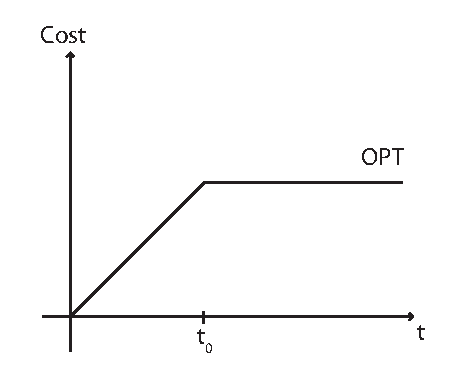
\includegraphics{Figures/Fig1}
	\caption{The optimal solution to the problem (cost in function of the time of the first request)} \label{fig1}
\end{figure}

It should be noted though that this algorithm is only theoritical~: it is not practical because it requires to know the value of $t_1$ to know what to do.

\paragraph{The best approximating deterministic algorithm}

Now a deterministic algorithm would have to decide a time $w$ at which it would shut down the hard drive and wait for the request if it's not arrived yet. For such an algorithm $A_w$, the cost graph is thus figure \ref{fig2} (there are two cases depending on whether $w$ is less or more than $y/x$).

\begin{figure}
	\centering
	\subfloat[Case when $w \leq y/x$]{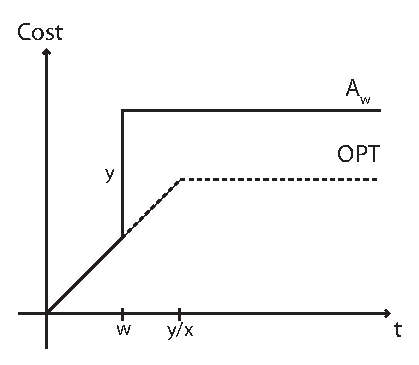
\includegraphics[width=6cm]{Figures/Fig2a}}
		\hspace{1cm}
	\subfloat[Case when $w \geq y/x$]{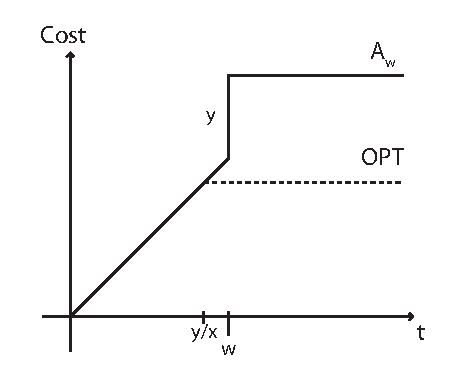
\includegraphics[width=6cm]{Figures/Fig2b}}
	\caption{The deterministic solution $A_w$ to the problem (optimal solution in strokes)} \label{fig2}
\end{figure}

\medskip

How good is such an algorithm compared to the optimal one~? We mesure that by calculating the approximation ratio~: $r = \max_t{\frac{cost(A_w, I_t)}{OPT_t}}$, where $cost(A_w, I_t)$ denotes the energy cost when using the algorithm $A_w$ if the request occurs at time $t$.

In the first case where $w \leq y/x$, we clearly have $r = \frac{x w + y}{x w} \geq 2$. Likewise, in the case where $w \geq y/x$, we have $r = \frac{x w + y}{y} \geq 2$.

This shows that any deterministic algorithm is at best a $2$-approximation of the optimal algorithm for solving the problem.

\smallskip

Moreover, by the previous expressions of $r$, we know that $A_{y/x}$ \emph{is} a $2$-approximation of the problem. So $A_{y/x}$ is the best approximating deterministic algorithm for our hard drive problem.

\medskip

If we go back to the real-life problem, this result means that without the use of randomness, one is doomed to use twice as much energy as optimally needed to run its hard drive.

Let's try to achieve a better result (on expectation) with a randomized algorithm.



\subsubsection{Using randomness to improve the algorithm}

\paragraph{Yao's Principle}

We will use Yao's principle on optimization problems, namely the following statement~:

\begin{theorem}
The cost of the best randomized algorithm on its worst instance is equal to the average cost of the best deterministic algorithm for the worst distribution of instances. More formally, 

\[ \min_p \max_q p A q = \max_q \min_p p A q\]

where $||p||_1=1, ||q||_1=1$ and $p,q \geq 0$
\end{theorem}

[See the notes on Yao's principle for more details about the notations and more insight on the meaning of this powerful principle.]


\paragraph{Application to the hard drive problem}

Here, we take as $A$ the following operator~: $C_{w,t} = \frac{cost(A_w, I_t)}{OPT_t}$, ie. the ratio on the instance $I_t$. The goal is to minimize this value, and Yao's principle provides a nice way to prove a lower bound on the competitive ratio of our problem.

Indeed, we have in particular that~:
\begin{equation} \label{eqn:yaomoitie}
\min_p \max_q p A q \quad \geq \quad \max_q \min_p p A q
\end{equation}

(which is actually the easy direction in Yao's principle). Following Yao's principle intuition, we can state that~: if $p$ is fixed, then $\max_q (pA)q$ can be seen as the worst case ratio of the randomized algorithm $pA$~; while when $q$ is fixed, $\min_p p(Aq)$ can be seen as the worst case ratio of the best deterministic algorithm on the distribution $q$.

Let's assume that we have found two distributions $p^\star$ and $q^\star$ such that $\max_q p^\star A q = \min_p p A q^\star$. Then by the inequality (\ref{eqn:yaomoitie}), it is clear that this value is actually the value $\min_p \max_q p A q = \max_q \min_p p A q$. And as the quantity $\max_q p^\star A q$ defines exactly the best randomized algorithm's competitive ratio, we have a lower bound on the best competitive ratio it is ever possible to achieve.

It is now time to actually find $p^\star$ and $q^\star$~: $p^\star$ provides the randomized algorithm, while the equality in (\ref{eqn:yaomoitie}) with the help of $q^\star$ proves that it is actually optimal.


\paragraph{$p^\star$ and $q^\star$}

Let us first simplify the notations to make computations easier. Without loss of generality, up to rescaling of time and cost, we can assume that $x=y=1$. We denote by $d$ the value of $w$ in this rescaled context. Then by definition, we have :

\begin{equation} \label{eq:eq1} \frac{cost(A_d,I_t)}{OPT_t} = \left\{\begin{array}{ll}
 \frac{d+1}{t}  & \text{ if }0 \leq d \leq t \leq 1 \\
 d+1 & \text{ if } 0 \leq d \leq t \text{ and } t >1 \\
 d & \text{ if } d >t>1 \\
 1 & \text{ otherwise } \end{array}\right. \end{equation}


This equation asks for two remarks.
\begin{itemize}
\item \textbf{First remark} : we can assume that $d \leq 1$ in the best deterministic algorithm (otherwise it would have been better to just shut down the hard drive to begin with).
\item \textbf{Second remark} : for $t >1$, the competitive ratio decreases, so we can assume that $t \leq 1$.
\end{itemize}

Now, looking at both these remarks and with some insight and some luck, let us guess the best randomized algorithm. The key is to think of an exponential distribution.

The "miracle" distribution is as follows. $d$ being a continuous value, the distribution is given by its density function : $p^\star(d) = \Pr_x(x \geq d)$

$$p^\star(d)= \left\{\begin{array}{ll} \frac{e^d}{e-1} & \text{if} \quad 0 \leq d \leq 1\\ 0 & \text{otherwise}\end{array}\right.$$

This is a density function since $\int_{\mathbb{R}} p^\star(d) d d = \int_0^1 \frac{e^d}{e-1}dd =1$.

Recall that the competitive ratio of a randomized algorithm is :

\[CR(A_{p^\star}) = \max_{t} \frac{ \mathbb{E}_{p^\star}(cost(A_{p^\star},I_t))}{OPT_t} \]


For a fixed $t$, this can be computed using equation (\ref{eq:eq1})~:

\begin{eqnarray*}
\frac{ \mathbb{E}_{p^\star}(cost(A_{p^\star},t))}{OPT_t}&=&\int_0^1 p^\star(d) CR(A_{d,t}) dd \\
&=& \int_0^t \frac{e^d}{e-1} \frac{d+1}{t}dd + \int_t^1 \frac{e^d}{e-1} 1 dd \\
&=& \frac{1}{e-1} ( \frac{1}{t} [e^t-1] + e-e^t + \frac{1}{t}\int_0^t de^d dd) \\
&=& \frac{e}{e-1}
\end{eqnarray*}

which is independent of $t$, and much less than 2 (about 1.4) ! This calculation provides us with a randomized algorithm of competitive ratio $\frac{e}{e-1}$.

\medskip

Now let us prove the lower bound. We need to find a distribution $q^\star$ such that no deterministic algorithm can beat this ratio, which will provide a lower bound using Yao's lemma as explained above.

Using again some insight and some luck, we propose the following miracle distribution~:

$$q^\star(t) = \left\{\begin{array}{ll} t \frac{e^{1-t}}{e-1} & \text{ if }  0\leq t <1 \\
0 & \text{ if } t >1\end{array}\right.$$

and $Pr(t=1) = \frac{1}{e-1}$.

Once again, this is a correct distribution since $\int_0^1 q^\star(t)dt + Pr(t=1)=\frac{e}{e-1}(-e^{-1} - e^{-1}+1)+\frac{1}{e-1}=\frac{-2+e+1}{e-1}=1$. 

To conclude, we just need to compute the average competitive ratio of any deterministic algorithm on this distribution, using equation (\ref{eq:eq1}) again :

\begin{eqnarray*}
E(\frac{cost(A_d,I_t)}{OPT_t}) &= &\int_0^d t \frac{e}{e-1}e^{-t}dt + \int_d^1 \frac{d+1}{t}t \frac{e}{e-1} e^{-t}dt + \frac{1}{e-1}(d+1)\\
&=& \frac{e}{e-1}(-de^{-d}-e^{-d}+1) + (d+1)\frac{e}{e-1}(e^{-1}-\frac{1}{e})\\
&=&\frac{e}{e-1}
\end{eqnarray*}

We conclude using Yao's Lemma that the randomized algorithm using the distribution $p^\star$ is optimal. This calculation is fairly tedious but otherwise the proof is simple, hence it makes a good example on how to prove lower bounds on randomized algorithms.

\bigskip

In the end, we found a (optimal) randomized algorithm which consumes on expectation only $40\%$ more energy than optimally necessary, instead of the $100\%$ we found in the deterministic case.





